% !TeX spellcheck = de_DE
\section{\ExercisePrefixMemory Debugging \optional}\label{sec:debugging}
\optionaltextbox

Die meisten Entwicklungsgebungen bieten Debuggingfunktionalität.
Debugging ermöglicht es schrittweise die Ausführung des Codes zu beobachten und lokale Variablen zu inspizieren und auf ihren aktuellen Wert zu prüfen. Oftmals ist diese Vorgehensweise gut geeignet kleinere Fehler in der Programmlogik zu finden.
Dazu kann man Breakpoints festlegen, an denen die Ausführung des Programms anhält.

Wir arbeiten in dieser Aufgabe mit einer absichtlich fehlerhaften Implementierung der einfachverketteten Liste (siehe \ref{sec:linkedList}).
Importiere dazu das Projekt unter folgendem Pfad: \cpppLinkToSampleSolution{debug_linked_lists}{debug\_linked\_lists}.

Diese setzt du in CodeLite mit einem Linksklick der Zeile in welcher der Ablauf stoppen soll wie in den Zeilen~8 und~12 in \Cref{fig:breakpoints}. 
Nutze für diese Aufgabe die Vorlage für das Debugging von \ref{sec:linked_list}. Starte den Debugger über \menuPath{Debugger \menuSep Start/Continue Debugger}.
Du wirst sehen, dass die Ausführung in Zeile 8 stoppt, was durch den grünen Pfeil markiert wird. Mit einem Klick auf den Continue-Button lässt sich der Programmablauf fortsetzen. Mit next wird die aktuelle Zeile ausgeführt und der Programmzeiger springt in die nächste Zeile. Step in bewirkt, dass in die erste Zeile der aufgerufenen Methode gesprungen wird. Step Out führt den Code bis zum Return-Statement aus und springt zurück und setzt den Programmzeiger hinter die aufgerufene Funktion. Im Fenster rechts unten (Abbildung \ref{fig:locals_view}) kannst du die Werte der Variablen inspizieren und solltest sehen, dass current\_size beim ersten Breakpoint den Wert 2 besitzt. Zudem kannst du während dem Debugging über einen Rechtsklick auf eine Zeile und "Run to here"  den Code bis zu dieser ausführen.
 
%Beispiel: linked list != Operator fehler einbauen und finden lassen. dabei vorgeben wo Breakpoint gesetzt werden soll und dann inspizieren lassen...
 
Setze nun in Zeile 25 von \lstinline{main.cpp} einen Breakpoint und versuche mit Hilfe des Debuggingmodus den Fehler zu finden, den ein tollpatschiger Programmierer hinterlassen hat.

\begin{figure}
	\centering
	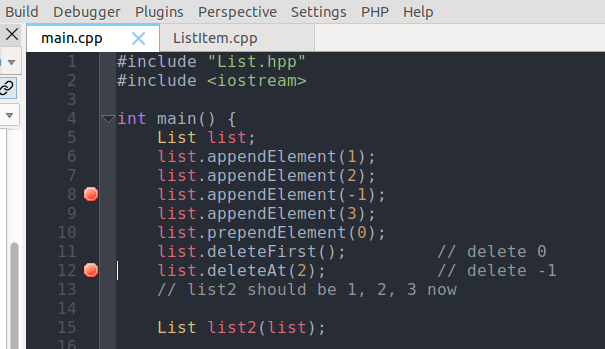
\includegraphics[width=.6\textwidth]{02_memory/figures/breakpoints.png}
	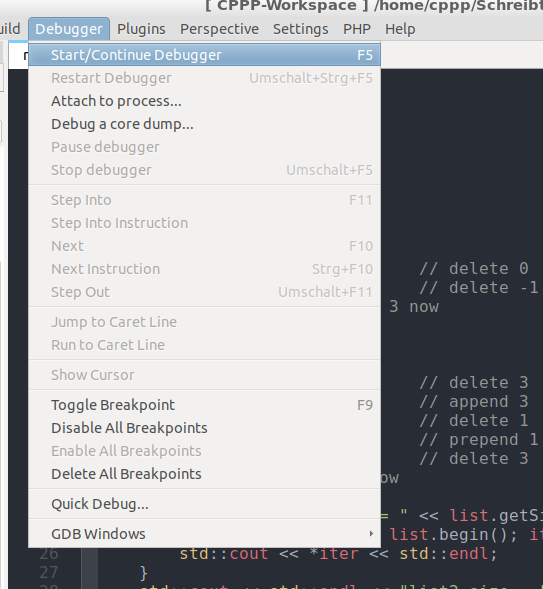
\includegraphics[width=.3\textwidth]{02_memory/figures/start_debugger.png}
	\caption{Setze Breackpoints und starte Debugger}
	\label{fig:breakpoints}
\end{figure}

%\begin{figure}
%	\centering
%	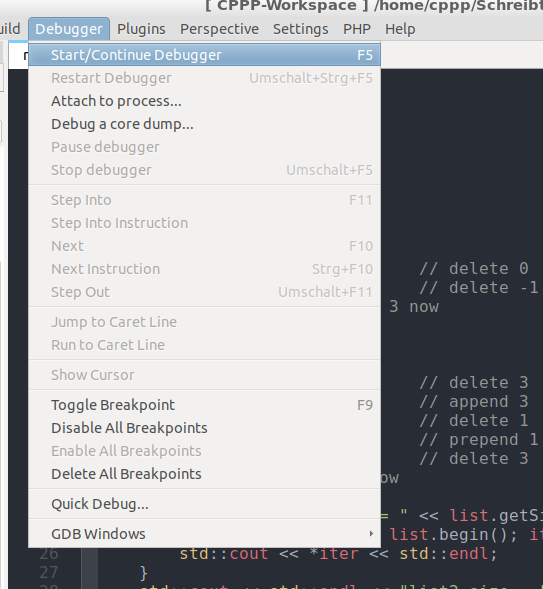
\includegraphics[width=.9\textwidth]{02_memory/figures/start_debugger.png}
%	\caption{Starte den Debugger}
%	\label{fig:start_debugger}
%\end{figure}

\begin{figure}
	\centering
	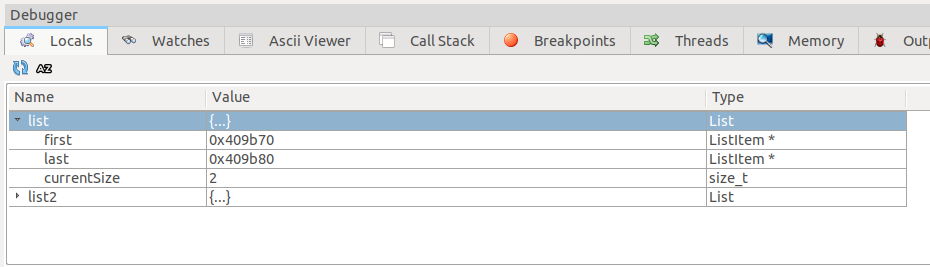
\includegraphics[width=.9\textwidth]{02_memory/figures/locals_view.png}
	\caption{Inspizieren von Variablen}
	\label{fig:locals_view}
\end{figure}

%\begin{figure}
%	\centering
%	
\includegraphics[width=.9\textwidth]{02_memory/figures/debugtools.png}
%	\caption{Debug Werkzeuge: }
%	\label{fig:debug_tools}
%\end{figure}

\hints{
	\item Mit step in kannst du auch die Aufrufe sehen, welche im For-Schleifenkopf gemacht werden.
}